\documentclass[english]{article}



\usepackage{graphicx}
\usepackage[hidelinks]{hyperref}
\usepackage{grffile}
\usepackage[T1]{fontenc}
\usepackage{babel}
\usepackage{float}
\usepackage{tabu}
\usepackage{ragged2e}
\usepackage{textcomp}
\usepackage{amstext}
\usepackage[final]{pdfpages}
\usepackage{caption}
\usepackage{color}


\graphicspath{{Pictures/}}


\begin{document}
	
	
	\begin{figure}[H]
		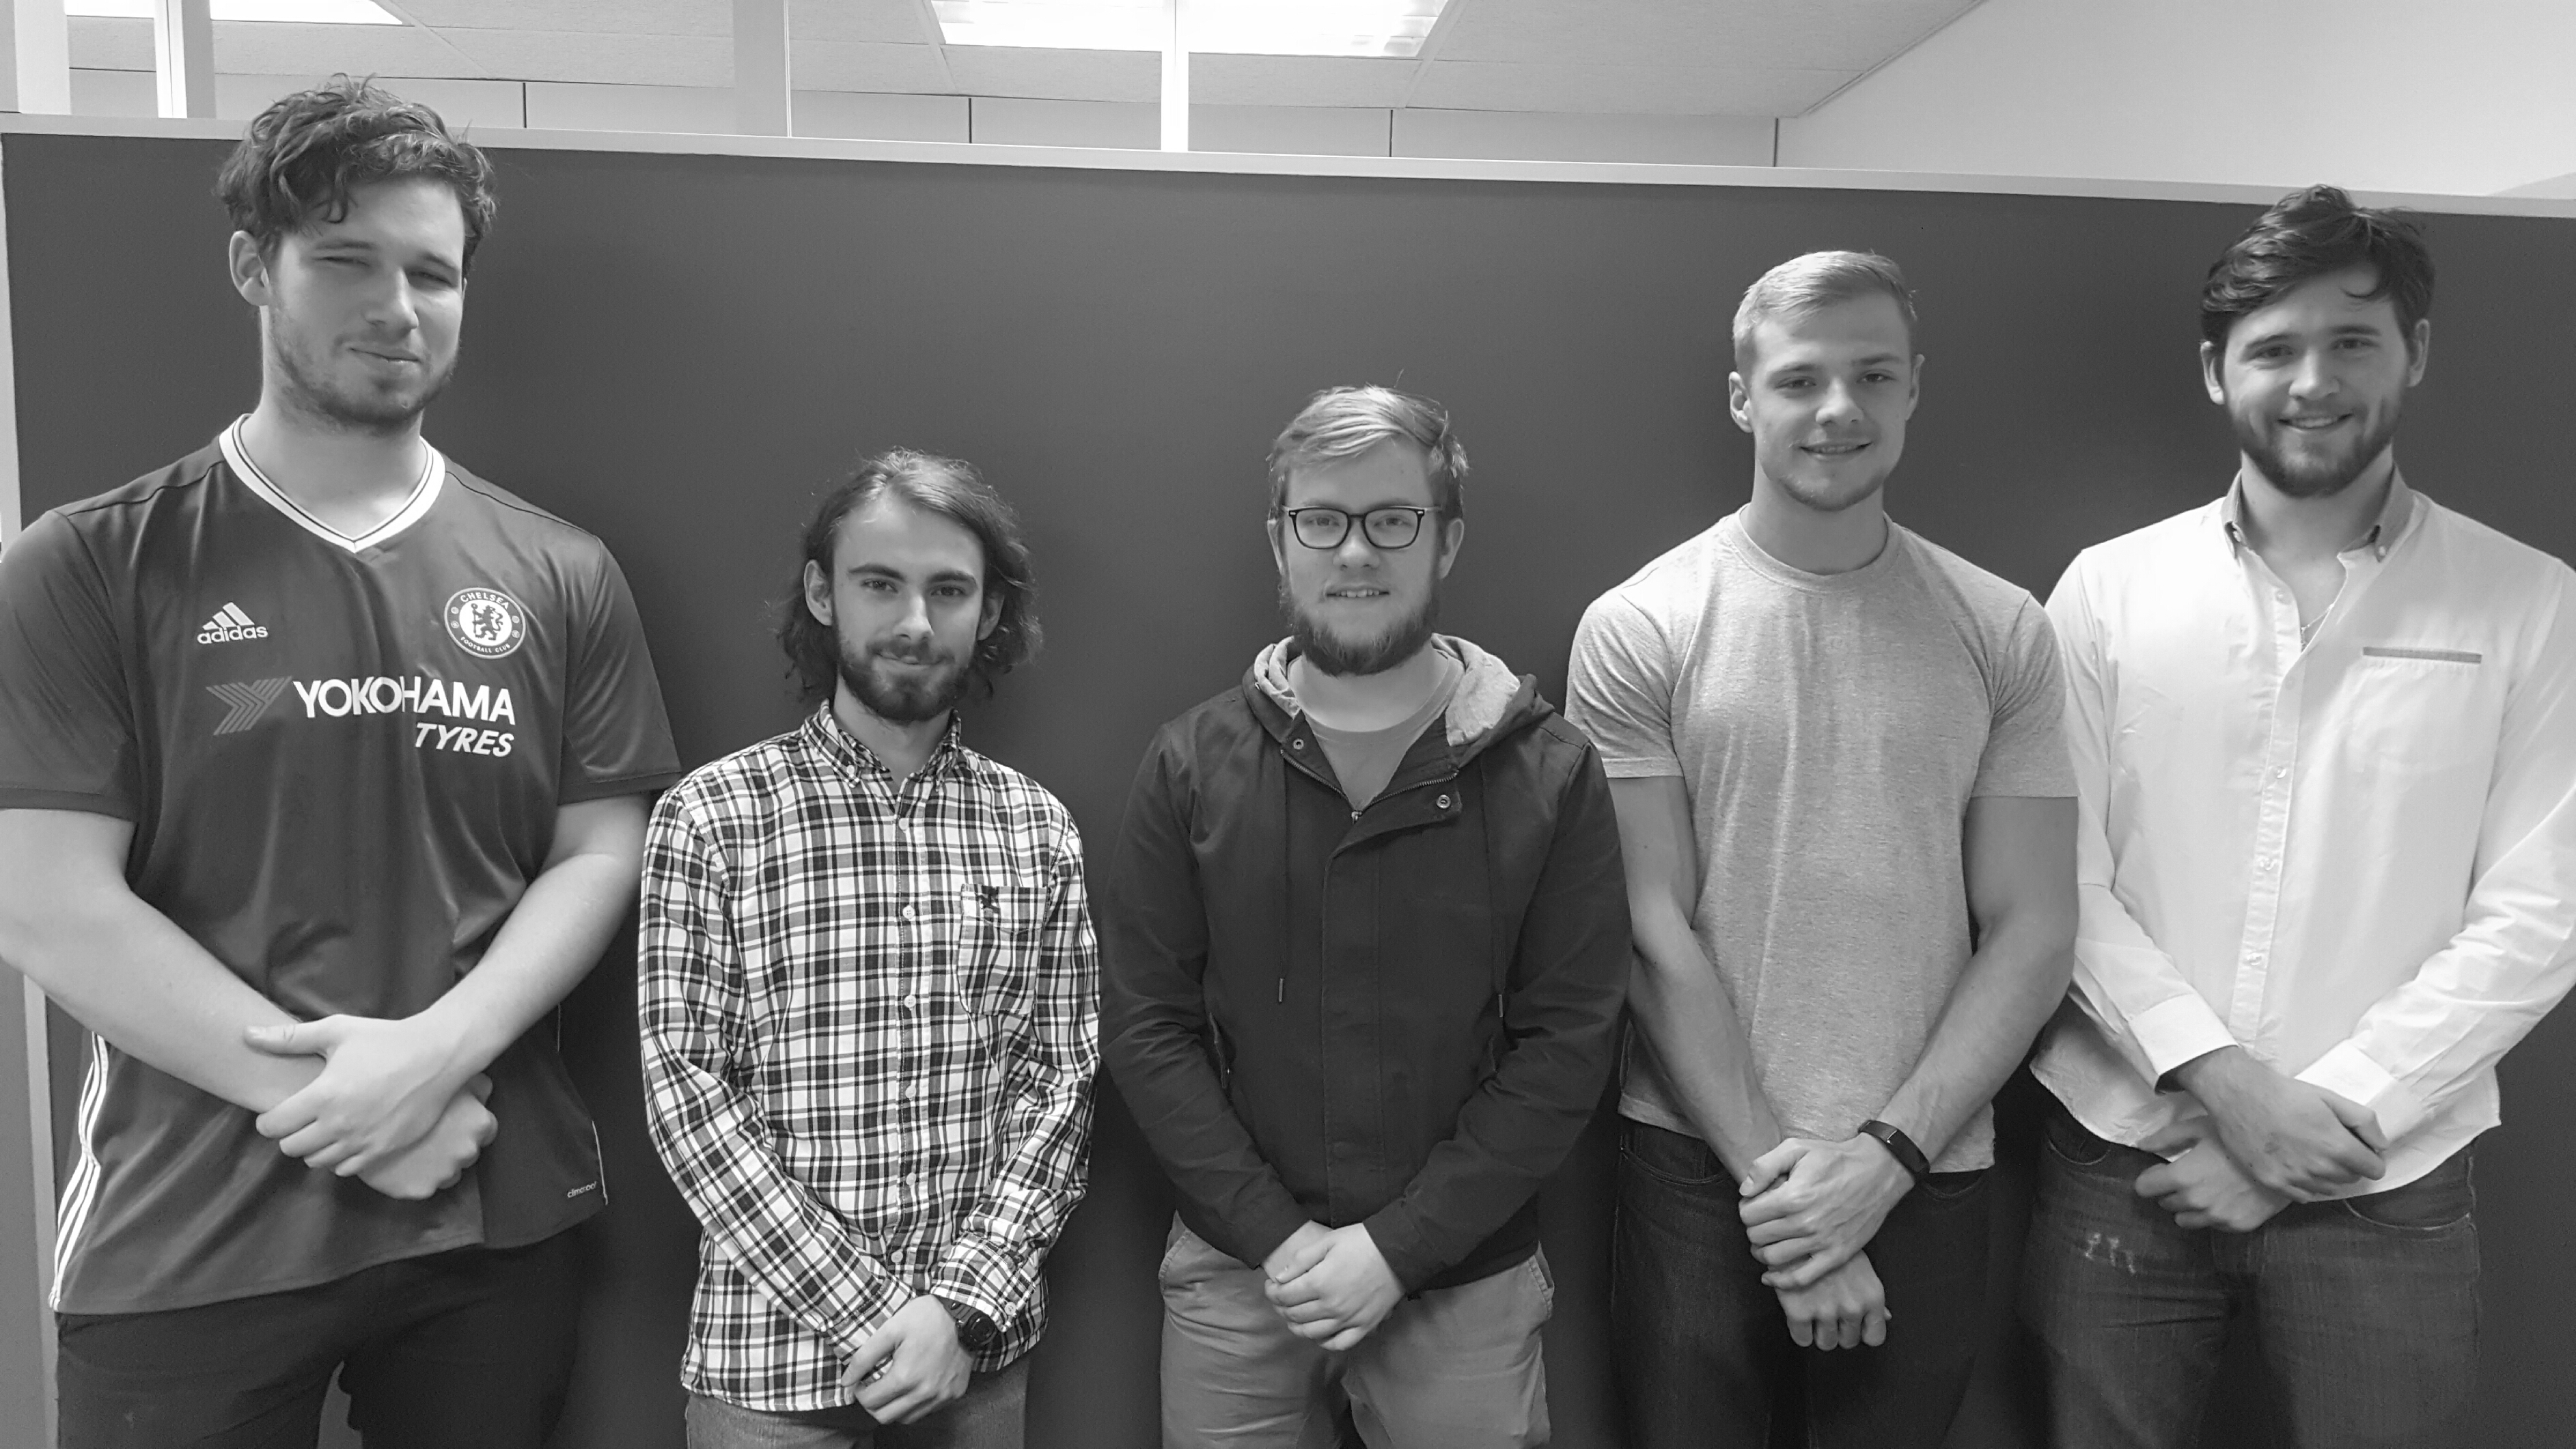
\includegraphics[width=\linewidth]{teamphoto.jpg}
	\end{figure}

	\begin{figure}[H]
		
\includegraphics[width=\linewidth]{teamtitle.jpg}
	\end{figure}

	\begin{figure}[H]
		
\includegraphics[width=\linewidth]{documenttitle.jpg}
	\end{figure}

	\begin{figure}[H]
		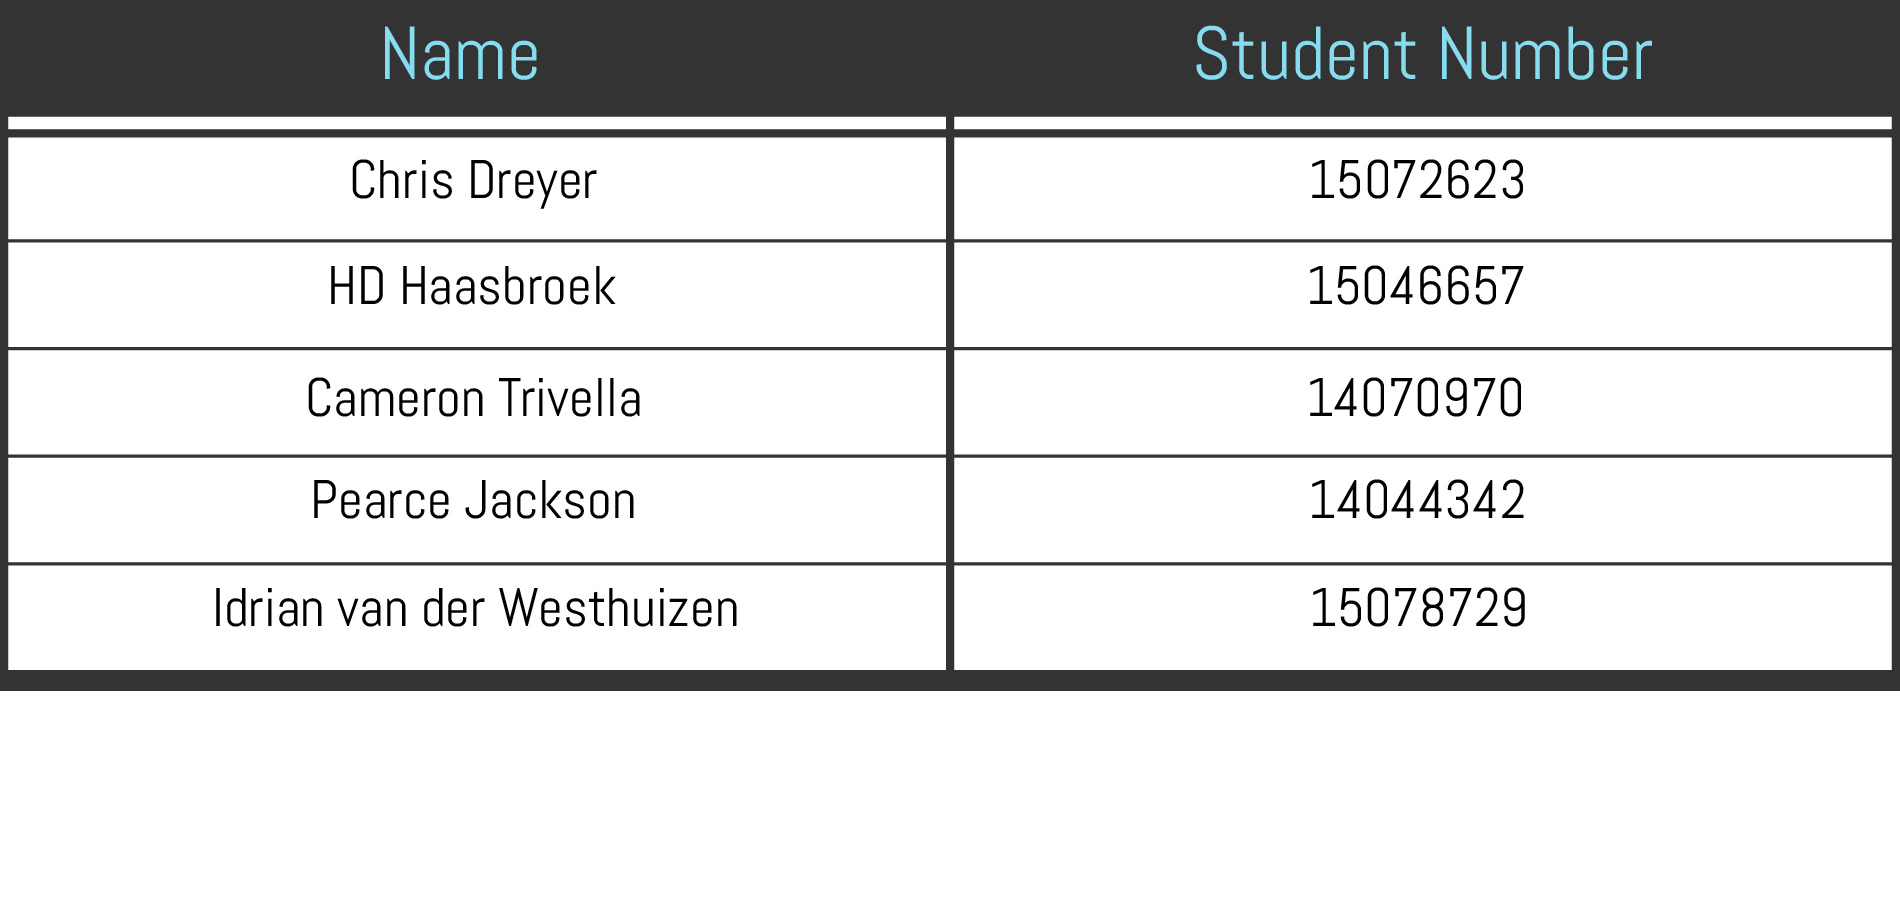
\includegraphics[width=\linewidth]{teamtable.jpg}
	\end{figure}
	
	\pagenumbering{gobble}
	\newpage
	\tableofcontents
	
	\pagenumbering{arabic}
	\newpage

	\section{Introduction}
	
		\subsection{Purpose}
		
		This SRS document aims to stipulate the requirements of the voxc.js library to aid in the development process and to ensure that a functional and usable product is delivered.
		
		\subsection{Product Scope}
		
		Voxc.js is meant to be an easy to use and easy to maintain JavaScript library, similar to how three.js is a library for WebGL. The purpose of the project is to provide users a way to import Voxel models into a webpage that would be using the Voxc.js library and use these Voxel models as a coordinate system to create newly genereated mesh object according to a rules file with a specified structure. The user will then be able to export the textured and rendered object.
		
		\subsection{References}
		
		\color{blue}
		\url{http://www.oskarstalberg.com/game/house/Index.html}
		\newline
		\\\url{https://voxel.codeplex.com/}
		\newline
		\\\url{https://pages.github.com/}
		\newline
		\\\url{http://threejs.org/}
		\newline
		\\\url{http://coffeescript.org/}
		\newline
		\\\url{http://es6-features.org/#Constants}
		\newline
		\\\url{http://www.typescriptlang.org/}
		\newline
		\\\url{http://www.codebelt.com/typescript/typescript-es6-modules-boilerplate/}
		\newline
		\\\url{http://giacomotag.io/typescript-webpack/}
		\color{black}
		
	\pagebreak
	
	\section{External Interface Requirements}
	
		\subsection{User Interfaces}
		The users should be able to interface with voxc.js through our web interface that will be hosted on Github Pages. They will mainly be using a laptop or a desktop to interface with the library. However the library itself should be able to interface with any website on any device with a web browser that has support for WebGL.
		\\\\
		This library should not require user profiles as their voxel objects are stored locally on browser storage and manipulated by the library. This implies that the user should only be led to one screen where they will be allowed to upload a voxel object file and a rules file if they choose to do so.
		
		\subsection{Software Interfaces}
		The system should incorporate several different languages in order to function. For the rules file, JSON objects should be 
		used so that the users can manipulate the file in any text editor based on set conventions and structure. 
		\\\\
		MagicVoxel should be used for the creation and manipulation of voxel objects. The library should be able to handle the .obj filetype for the voxel objects.
		\\\\
	 	The library should use TypeScript as the JavaScript variant to enable future developers and current developers to debug easier. The library should run on all major internet browsers that support WebGL.
		
		\subsection{Communications Interfaces}
		HTTP will be used to handle GET and POST requests and FTP will be used for file uploads and downloads.
	\pagebreak
	
	\section{System Features}
	
		\subsection{System Feature 1}
		
			 \subsubsection{Description and Priority}
			 
			 \subsubsection{Stimulus/Response Sequences}
			 
			 \subsubsection{Functional Requirements}
			 
	\pagebreak
	
	\section{Other Nonfunctional Requirements}
	
		\subsection{Performance Requirements}
		\subsubsection {Time to respond to an uploaded file}
		A user is required to upload a voxel object to the library and then should be allowed to mainpulate a rules file if they choose to do so or they should be able to use a predefined rules file such that the rules are applied to the object. The library must not delay once a file is uploaded, this means the time it takes to respond to a uploaded file should be proportional to the files size.
		
		\subsubsection{Respond to user interaction}
		The system should respond to user interactions in real time.
		
		\subsubsection{Reliability}
		The system should never cease working completely unless the error is caused by external systems outside our control (operating system, web APIs, etc). Ideally an entire system uptime (per month) of 99.0\% must be reached, meaning that the system should have validation and error checking to prevent unwanted results.
		
		\subsubsection{Maintainability}
		The library's code must be well documented, both by means of in-code comments and external documentation, to aid in 
		maintaining the system. A user manual should also be provided to make it easier to understand and ultimately maintain the library.
		
		\subsubsection{Portability}
		This library should be accessible across all major internet browsers that support WebGL. These include Chrome, Firefox etc.
		The library should also be able to be imported to any website.
		
		\subsubsection{Scalibilty}
		The system should be able to handle the majority of web browsers and file sizes, by file size we mean that the system should not necessarily struggle or outright reject a file because it was too large. Realistically we cannot handle all file sizes, but the system should aim to handle a large as possible file size. 
		\\\\
		Additionally the library should be able to work with any other webpage as a simple imported library, therefore users should be able to alter positions and perhaps even sizes of the dom elements used to upload, download and display the objects.
		
		\subsubsection{Usability}
		The Voxel library should be easy to operate and understand. The core functions of the system shouldn't take the user more 
		than a minute to access and understand. A user manual should be provided to aid in the use of the library and to explain some advanced functions or settings.
		
		\subsection{Security Requirements}
		This library should be an open source project and so the code will be freely available to anyone visiting the Github repository. The actual web interface hosted on Github will act as a demo of the library and should be protected, the only editing that a user should be able to do is uploading of objects and editing their own rules file.
		
		\subsection{Quality Requirements}
		*Stars for reviewing*
		
	\pagebreak
	
\end{document}
